\documentclass[tikz,border=2pt]{standalone}
\usepackage{amsmath}
\begin{document}
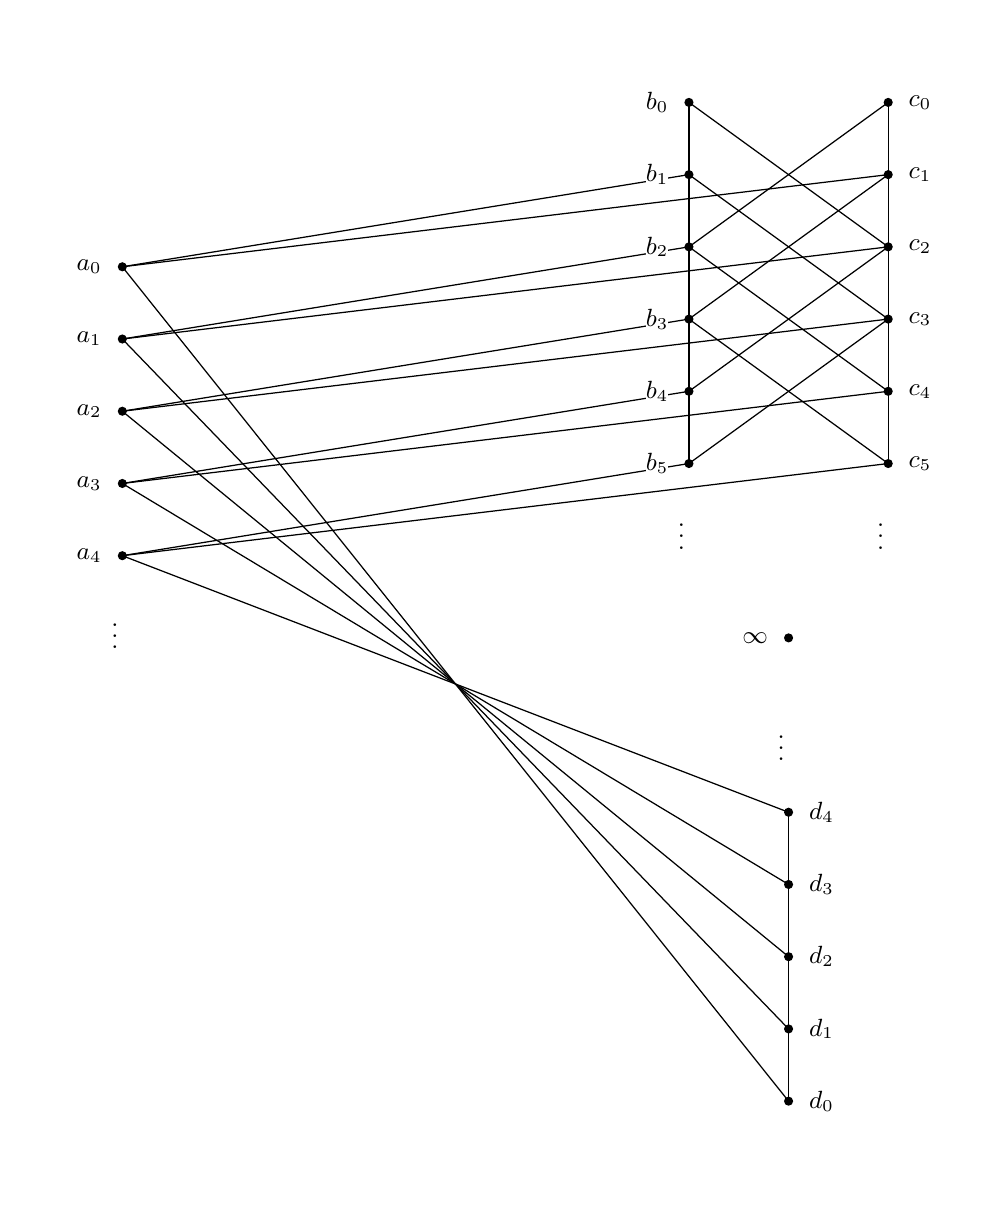
\begin{tikzpicture}[x=.45pt,y=-.45pt,line width=.45pt,line cap=round,font=\fontsize{9}{10}\selectfont]
\path[use as bounding box] (99,20) rectangle (860,952);
\coordinate (nb0) at (630,80);
\coordinate (nc0) at (790,80);
\coordinate (nb1) at (630,138);
\coordinate (nc1) at (790,138);
\coordinate (nb2) at (630,196);
\coordinate (nc2) at (790,196);
\coordinate (nb3) at (630,254);
\coordinate (nc3) at (790,254);
\coordinate (nb4) at (630,312);
\coordinate (nc4) at (790,312);
\coordinate (nb5) at (630,370);
\coordinate (nc5) at (790,370);
\coordinate (na0) at (175,212);
\coordinate (na1) at (175,270);
\coordinate (na2) at (175,328);
\coordinate (na3) at (175,386);
\coordinate (na4) at (175,444);
\coordinate (ninfinity) at (710,510);
\coordinate (nd0) at (710,882);
\coordinate (nd1) at (710,824);
\coordinate (nd2) at (710,766);
\coordinate (nd3) at (710,708);
\coordinate (nd4) at (710,650);
\draw (nb1) -- (nb0);
\draw (nc1) -- (nc0);
\draw (nb2) -- (nb1);
\draw (nc2) -- (nc1);
\draw (nb2) -- (nc0);
\draw (nc2) -- (nb0);
\draw (nb3) -- (nb2);
\draw (nc3) -- (nc2);
\draw (nb3) -- (nc1);
\draw (nc3) -- (nb1);
\draw (nb4) -- (nb3);
\draw (nc4) -- (nc3);
\draw (nb4) -- (nc2);
\draw (nc4) -- (nb2);
\draw (nb5) -- (nb4);
\draw (nc5) -- (nc4);
\draw (nb5) -- (nc3);
\draw (nc5) -- (nb3);
\draw (na0) -- (nb1);
\draw (na0) -- (nc1);
\draw (na1) -- (nb2);
\draw (na1) -- (nc2);
\draw (na2) -- (nb3);
\draw (na2) -- (nc3);
\draw (na3) -- (nb4);
\draw (na3) -- (nc4);
\draw (na4) -- (nb5);
\draw (na4) -- (nc5);
\draw (nd0) -- (na0);
\draw (nd1) -- (na1);
\draw (nd0) -- (nd1);
\draw (nd2) -- (na2);
\draw (nd1) -- (nd2);
\draw (nd3) -- (na3);
\draw (nd2) -- (nd3);
\draw (nd4) -- (na4);
\draw (nd3) -- (nd4);
\node at (169,502) {$\vdots$};
\node at (624,422) {$\vdots$};
\node at (784,422) {$\vdots$};
\node at (704,592) {$\vdots$};
\fill (nb0) circle[radius=1.65pt];
\node[anchor=east,inner sep=0pt,fill=white] at (614,80) {$b_{0}$};
\fill (nc0) circle[radius=1.65pt];
\node[anchor=west,inner sep=0pt,fill=white] at (806,80) {$c_{0}$};
\fill (nb1) circle[radius=1.65pt];
\node[anchor=east,inner sep=0pt,fill=white] at (614,138) {$b_{1}$};
\fill (nc1) circle[radius=1.65pt];
\node[anchor=west,inner sep=0pt,fill=white] at (806,138) {$c_{1}$};
\fill (nb2) circle[radius=1.65pt];
\node[anchor=east,inner sep=0pt,fill=white] at (614,196) {$b_{2}$};
\fill (nc2) circle[radius=1.65pt];
\node[anchor=west,inner sep=0pt,fill=white] at (806,196) {$c_{2}$};
\fill (nb3) circle[radius=1.65pt];
\node[anchor=east,inner sep=0pt,fill=white] at (614,254) {$b_{3}$};
\fill (nc3) circle[radius=1.65pt];
\node[anchor=west,inner sep=0pt,fill=white] at (806,254) {$c_{3}$};
\fill (nb4) circle[radius=1.65pt];
\node[anchor=east,inner sep=0pt,fill=white] at (614,312) {$b_{4}$};
\fill (nc4) circle[radius=1.65pt];
\node[anchor=west,inner sep=0pt,fill=white] at (806,312) {$c_{4}$};
\fill (nb5) circle[radius=1.65pt];
\node[anchor=east,inner sep=0pt,fill=white] at (614,370) {$b_{5}$};
\fill (nc5) circle[radius=1.65pt];
\node[anchor=west,inner sep=0pt,fill=white] at (806,370) {$c_{5}$};
\fill (na0) circle[radius=1.65pt];
\node[anchor=east,inner sep=0pt,fill=white] at (159,212) {$a_{0}$};
\fill (na1) circle[radius=1.65pt];
\node[anchor=east,inner sep=0pt,fill=white] at (159,270) {$a_{1}$};
\fill (na2) circle[radius=1.65pt];
\node[anchor=east,inner sep=0pt,fill=white] at (159,328) {$a_{2}$};
\fill (na3) circle[radius=1.65pt];
\node[anchor=east,inner sep=0pt,fill=white] at (159,386) {$a_{3}$};
\fill (na4) circle[radius=1.65pt];
\node[anchor=east,inner sep=0pt,fill=white] at (159,444) {$a_{4}$};
\fill (ninfinity) circle[radius=1.65pt];
\node[anchor=east,inner sep=0pt,fill=white] at (694,510) {$\infty$};
\fill (nd0) circle[radius=1.65pt];
\node[anchor=west,inner sep=0pt,fill=white] at (726,882) {$d_{0}$};
\fill (nd1) circle[radius=1.65pt];
\node[anchor=west,inner sep=0pt,fill=white] at (726,824) {$d_{1}$};
\fill (nd2) circle[radius=1.65pt];
\node[anchor=west,inner sep=0pt,fill=white] at (726,766) {$d_{2}$};
\fill (nd3) circle[radius=1.65pt];
\node[anchor=west,inner sep=0pt,fill=white] at (726,708) {$d_{3}$};
\fill (nd4) circle[radius=1.65pt];
\node[anchor=west,inner sep=0pt,fill=white] at (726,650) {$d_{4}$};
\end{tikzpicture}
\end{document}
